% ============================================================================
% AntMill - AAAI-27 anonymous submission draft (v0.2, 2026-07-12)
% Built on AuthorKit27 (aaai2027.sty, template version 2027.1).
% Compile: pdflatex -> bibtex -> pdflatex -> pdflatex
% Before submission: confirm conference page limits and submit the required
% reproducibility checklist and anonymized supplementary artifact.
% ============================================================================
\documentclass[letterpaper]{article} % DO NOT CHANGE THIS
\usepackage[submission]{aaai2027}  % DO NOT CHANGE THIS
\usepackage[hyphens]{url}  % DO NOT CHANGE THIS
\usepackage{graphicx} % DO NOT CHANGE THIS
\urlstyle{rm} % DO NOT CHANGE THIS
\def\UrlFont{\rm}  % DO NOT CHANGE THIS
\usepackage{natbib}  % DO NOT CHANGE THIS AND DO NOT ADD ANY OPTIONS TO IT
\usepackage{caption} % DO NOT CHANGE THIS AND DO NOT ADD ANY OPTIONS TO IT
\frenchspacing  % DO NOT CHANGE THIS
\usepackage{booktabs}
\usepackage{amsmath}
\pdfinfo{
/TemplateVersion (2027.1)
}

\setcounter{secnumdepth}{2}

\title{Locally Plausible, Globally Wasteful: Consensus Consolidation Can Degrade Shared Experience in Multi-Agent LLM Systems}
\author{Anonymous Submission}
\affiliations{}

\begin{document}
\maketitle

\IfFileExists{generated/revision_results/revision_macros.tex}{
  \input{generated/revision_results/revision_macros.tex}
}{
  \typeout{Revision macros are pending complete formal evidence.}
}

\begin{abstract}
Multi-agent LLM systems increasingly share experiential memory: agents write distilled
insights into a common pool that is retrieved and injected into every teammate's context. We
study a controlled failure mode of one such design that requires no wrong facts, no poisoned
text, and no illegal actions. In a trap-maze microscope where every route is legal and
shortest-path cost is exactly measurable, we run a preregistered ladder of experiments using
implementations based on published components (ExpeL-style insight operations and
Generative-Agents-style retrieval). Across a five-arm multi-agent matrix, active memory
degrades efficiency and amplifies looping; under our shared-consolidated protocol, the effect
is largest relative to the write-only frozen control (success-only excess steps $+11.8$, 95\%
CI $[7.7,16.0]$; loop rate $+0.138$, CI $[0.092,0.188]$; $5/5$ seed signs) and its loop
amplification is the only one that significantly exceeds private memory. We do not observe the
preregistered read-side importance dose-response; a write-side audit instead finds that
consolidation compresses the active strategy supply by ${\sim}2.3\times$. The effect persists
without self-healing over $T{=}10$, whereas the exploratory $\lambda{=}1$ append arm improves
over that horizon. Two archive interventions bound, but do not identify, the mechanism:
re-exposure at added dose worsens stagnation, and the equal-dose arm fails its preregistered
diversity-expansion check. A Qwen3-32B probe replicates compression but leaves the efficiency effect
unresolved and excludes a loop amplification of the primary model's magnitude. These results
identify a bounded risk in a measurable setting rather than a task- or model-universal failure.
\end{abstract}

% ============================================================================
\section{Introduction}
% ============================================================================

When army ants lose the pheromone trail, each ant follows the locally impeccable rule
``follow the ant in front of you,'' and the colony organizes itself into a circular mill that
marches until exhaustion. No single step is wrong; the composition is fatal.

We test whether shared experiential memory in multi-agent LLM systems can admit an analogous
failure. The prevailing design pattern---popularized for single agents by
experiential learners such as ExpeL~\citep{zhao2024expel} and
Reflexion~\citep{shinn2023reflexion}, and extended to agent teams by experiential
co-learning~\citep{qian2024colearning} and cross-task multi-agent experience
pools~\citep{li2025mael}---lets agents distill natural-language insights from their own
trajectories, store them in a memory pool, and retrieve them as guidance. When the pool is
\emph{shared} and a reviewer LLM \emph{consolidates} it by merging, editing, and
up/down-voting insights, every ingredient is individually reasonable and individually
published. We test whether their composition has measurable costs.

The failure we test is \emph{silent}. Agents can keep succeeding, never cross walls, and never
submit false answers; the experience text is locally plausible and derived from genuine
trajectories. Yet routes can grow longer, agents can revisit the same cells, and loop
signatures can rise. Because no error is emitted, success alone need not expose this loss.

Studying such a compositional failure on a live benchmark confounds every knob at once. We
instead build a \emph{mechanism microscope}: a generated $15\times15$ trap-maze family with
known shortest paths, local observations, and a step cap, in which efficiency loss and
looping are exactly measurable per route (Figure~\ref{fig:fig1}). Into this microscope we
place concrete implementations of published component families
(Table~\ref{tab:components}). This isolates the tested composition---shared memory plus
reviewer consolidation---from maze observability and route-cost ambiguity; it does not make
the maze result a substitute for deployment evaluation. All confirmatory experiments were
preregistered with frozen gates; every deviation and negative result appears in an append-only
log.

Our contributions:
\begin{itemize}
\item \textbf{A preregistered phenomenon in a controlled setting.} In a five-arm memory
matrix over five seeds, the shared-consolidated arm degrades success-only route efficiency,
amplifies loops, and reduces success relative to a write-only frozen control. Relative to
\emph{private} memory, the shared-specific separation is loop amplification, not a broad
efficiency gap.
\item \textbf{Protocol-level factor separation.} Fresh controls compare joint shared
consolidation with per-agent consolidation, fixed-capacity append/agree, read-side MMR, and an
exact round-by-round candidate-supply yoke. A prespecified sensitivity envelope varies
retrieval capacity, pool cap, reviewer budget, merge threshold, and recency. Together these
separate sharing, consolidation, candidate count, and retrieval policy as far as the tested
protocols permit, without treating any single contrast as full causal isolation.
\item \textbf{A bounded mechanism account.} The preregistered read-side importance
dose-response is not supported, while a write-side audit shows a ${\sim}2.3\times$
compression of active strategy supply. Archive interventions and the new factor controls
constrain supply compression as a candidate channel rather than identify it as the cause.
\item \textbf{Model and task-level boundaries.} A Qwen3-32B probe tests cross-model transfer,
and a preregistered six-family BrowserGym MiniWoB study tests executable browser interaction.
The latter uses an equal-family, seed-clustered gate with explicit replication, not-detected,
and quality-withheld branches rather than assuming transfer from the maze.
\item \textbf{A reusable microscope and discipline.} The anonymized supplementary artifact
contains the environment, runners, prompts, configurations, paired-route statistics,
sanitizer, memory audits, and preregistrations with freeze hashes.
\end{itemize}

\begin{figure*}[t]
\centering
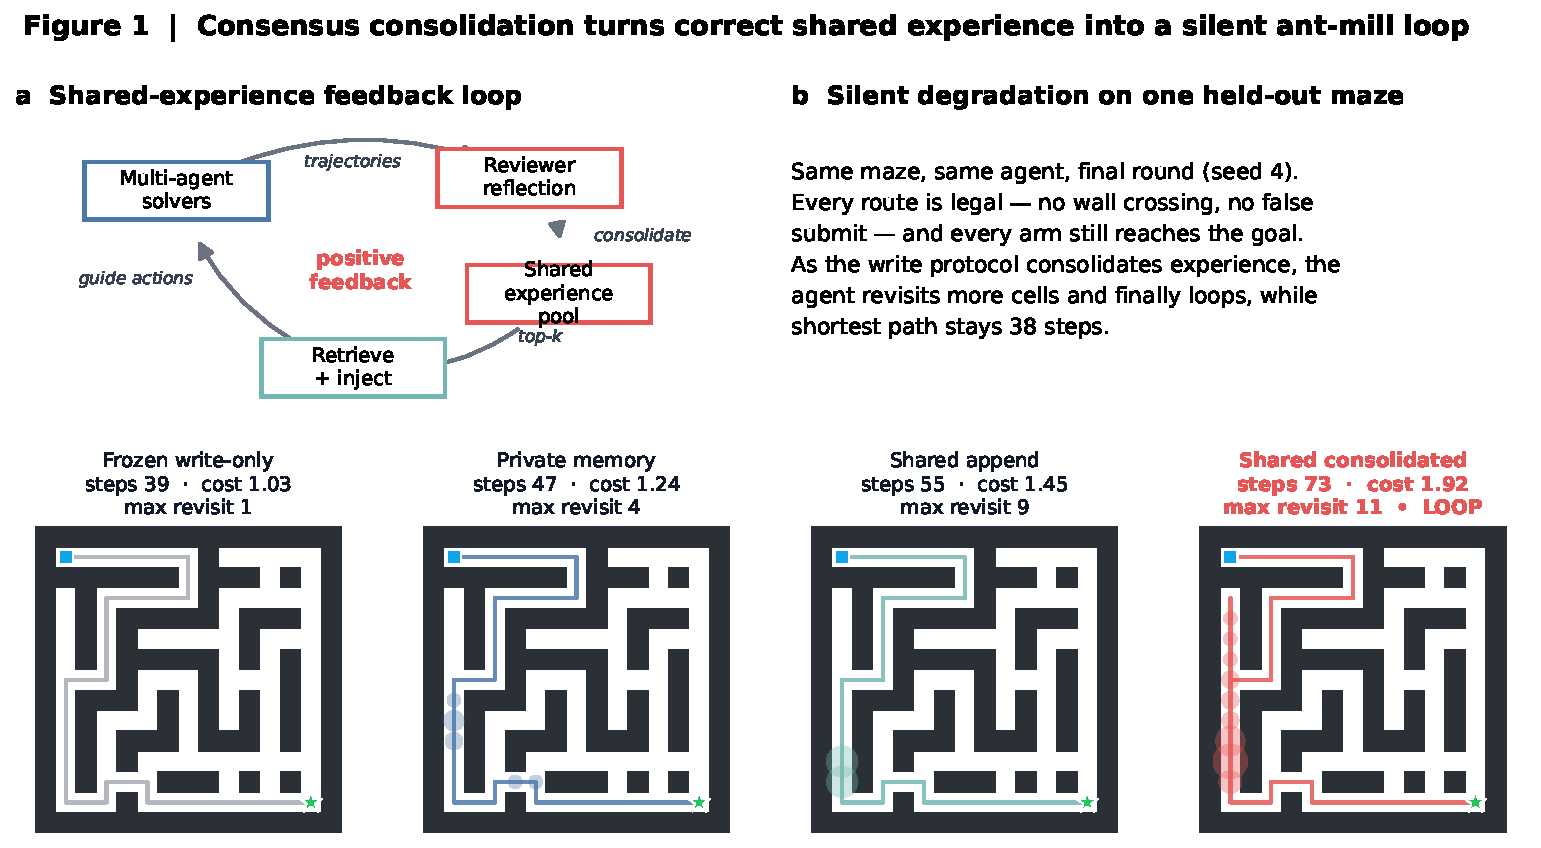
\includegraphics[width=0.92\textwidth]{figures/beta/figure1_mechanism.pdf}
\caption{\textbf{Mechanism microscope and a silent degradation case.} (a)~The
shared-experience feedback loop: solver trajectories are reflected into a shared pool,
consolidated by LLM-issued operations, retrieved top-$k$, and injected back as guidance---a
positive-feedback cycle. (b)~Same held-out maze and agent, final round; shortest path 38.
Revisit heat grows as the write protocol consolidates, culminating in a silent loop under
shared-consolidated memory, while every route stays legal and successful.}
\label{fig:fig1}
\end{figure*}

% ============================================================================
\section{Related Work}
% ============================================================================

\paragraph{Single-agent experiential learning.}
ExpeL~\citep{zhao2024expel} distills insights from success/failure trajectories with
ADD/EDIT/UPVOTE/DOWNVOTE operations and retrieves them as guidance;
Reflexion~\citep{shinn2023reflexion} converts failures into verbal self-corrections;
ReAct~\citep{yao2023react} interleaves reasoning and acting; Generative
Agents~\citep{park2023generative} score memories by relevance, importance, and recency;
MemoryBank~\citep{zhong2024memorybank} adds long-term memory management. These works
established that experience helps a \emph{single} agent. Our write operations, retrieval
scoring, and distillation prompts follow their component families
(Table~\ref{tab:components}); we do not claim implementation-identical reproductions of the
full original systems.

\paragraph{Multi-agent experience sharing.}
Experiential co-learning~\citep{qian2024colearning} shares shortcut experiences between
instructor and assistant agents in ChatDev~\citep{qian2024chatdev};
MAEL~\citep{li2025mael} equips each agent in a collaboration graph with an experience pool
queried by similarity and reward; multi-agent debate~\citep{du2024debate} and
self-consistency~\citep{wang2023selfconsistency} aggregate opinions rather than memories;
MetaGPT~\citep{hong2024metagpt} shares a message pool. All published sharing designs
accumulate experience additively. To our knowledge, no prior work evaluates the natural next
step---\emph{LLM-driven consensus consolidation of a shared experience pool}---with controls;
that protocol is exactly our subject.

\paragraph{Memory risk and governance.}
Recent work studies failure modes in LLM memory systems~\citep{garg2026memfail} and
longitudinal risks of memory-equipped agents~\citep{wang2026remembering}. We complement this
line with a preregistered, controlled study of one specific protocol---shared reviewer
consolidation---with exact route-level ground truth and explicitly reported negative
interventions.
For the task-level boundary beyond the maze, MiniWoB from World of
Bits~\citep{shi2017worldofbits}, exposed through
BrowserGym~\citep{chezelles2024browsergym}, supplies reproducible browser-interaction
tasks. We use six families as a controlled transfer boundary, not as evidence
about live-web deployment. MemoryArena instead evaluates memory across interdependent
multi-session agent tasks~\citep{he2026memoryarena}; our exact-ground-truth microscope
trades that breadth for mechanism visibility.

\paragraph{Applicability and governance controls.}
A complementary line treats memory use as a control decision rather than an unconditional
retrieval step. Lu et al.\ gate memory exposure and selectively accept memory-conditioned
answers~\citep{lu2026tag}; MemArchitect places policy-based adjudication between an agent and
its memory store~\citep{kumar2026memarchitect}; and ProactAgent learns when retrieval is
worth invoking during an interaction~\citep{cai2026proactagent}. These are not direct
baselines for our fixed shared-pool protocol: they add routing, acceptance, or governance
policies that our microscope deliberately holds absent. Our contribution is instead a
controlled failure characterization that motivates testing such controls against strategy
supply, loops, and stagnation, not only task success.
RAP likewise retrieves context-matched past experience for planning rather than exposing
one globally consolidated pool~\citep{kagaya2024rap}; this selective design is a natural
comparison point for the diversity-aware retrieval tested here.

% ============================================================================
\section{The Maze Microscope}\label{sec:method}
% ============================================================================

\begin{table}[t]
\centering
\small
\caption{Concrete mechanisms adapted from published component families. We retain their
operation family or retrieval objective; the shared reviewer update is the evaluated
composition, not an implementation-identical reproduction of any full prior system.}
\label{tab:components}
\begin{tabular}{@{}p{0.58\columnwidth}@{\hspace{4pt}}p{0.34\columnwidth}@{}}
\toprule
Component & Source \\
\midrule
Insight ops \textsc{add}/\textsc{edit}/\textsc{up}/\textsc{down}, importance-0 deletion & ExpeL \\
Retrieval scoring (relevance{+}importance{+}recency, $\lambda$) & Generative Agents \\
Insight distillation from trajectories & ExpeL \\
Stepwise solving with injected experience & ReAct-style \\
Shared pool across agents & Co-learning, MAEL \\
One reviewer update over a shared pool & \textbf{composition under test} \\
\bottomrule
\end{tabular}
\end{table}

\paragraph{Environment.}
We generate a $15\times15$ ``trap'' maze family with enforced shortest-path length $\geq 30$
and disjoint train/heldout splits per experiment seed. Solvers receive local observations
only (no maze graph, no shortest path), act under a 120-step cap, and are scored by exact
excess steps over the known optimum. Efficiency loss and loop signatures are therefore
measurable per route---the property that makes silent degradation visible at all.

\paragraph{System under test.}
Four solver agents attempt the \emph{same} tasks in independent environment copies. They
never communicate or vote; the \emph{only} coupling channel is the experience memory. Each
round $t$ comprises (i)~evaluation on 12 heldout mazes per agent (48 routes) and
(ii)~a training batch of 4 mazes per agent (16 routes). In the shared-consolidated
reference, each training maze then produces one reviewer call over the four agent logs and
the shared pool. The private-consolidated control instead invokes the same operation grammar
separately for each agent's single log and private pool: four calls per training maze, each
with a six-operation cap, versus one six-operation shared call. This preserves the
no-cross-agent-memory intervention but does not equalize reviewer-call or total operation
opportunity, so shared versus private is a protocol-level contrast rather than a one-factor
causal estimate of sharing alone. The reviewer sees only batched logs and quality
signals---never hidden routes. We use ``consensus'' operationally for the one joint shared
reviewer update, not for a solver vote or multi-agent dialogue. The final round evaluates
without writing. Retrieval injects the top-$k{=}6$ insights; the pool is capped at 80.

\paragraph{Protocol detail.}
In the consolidated arm, the reviewer emits at most six JSON
\textsc{add}/\textsc{edit}/\textsc{upvote}/\textsc{downvote} operations over the visible
pool. New items begin with two votes; zero-vote items are removed; near-duplicate additions
are merged at a fixed similarity threshold. In E2, relevance-only top-$k$ retrieval uses
Generative-Agents-style normalization with importance weight $\lambda{=}0$ and recency weight
zero. E3 changes only $\lambda$. Full prompts, configurations, sanitizer rules, and retry
behavior are included in the anonymized supplementary artifact.

\paragraph{Arms.}
The five-arm matrix decomposes ``multi-agent shared consolidated memory'' factor by factor:
\texttt{no-memory} (is multi-agent execution itself pathological?); \texttt{frozen} (reviewer
writes, solvers never read: is \emph{storage} harmful?); \texttt{private} (per-agent pools:
the same operation grammar consolidates each agent's own pool, but no item crosses agents;
reviewer calls are allocated per pool as noted above); \texttt{shared-append} (each agent's
distilled reflections enter one shared pool; near-duplicate additions receive a deterministic
agreement upvote, but there is no joint reviewer-issued \textsc{edit} or
\textsc{downvote}); and \texttt{shared-consolidated} (the protocol under test).

\paragraph{Fresh mechanism and robustness suites.}
On fresh caches, the five-seed control suite compares shared consolidation with
private consolidation, fixed-capacity append/agree (cap 14), and MMR retrieval. MMR
greedily reranks GA candidates with $0.70\,s_{\mathrm{GA}}-0.30$ times maximum
redundancy, where redundancy is cosine similarity between deterministic
128-dimensional token-hashing embeddings; it changes read selection only. A separate
append/agree arm is yoked, for every seed and round, to the candidate-pool size produced by
shared consolidation; its schedule is extracted without reading behavioral fields.
The three-seed one-factor sensitivity suite varies
$k\in\{3,6,10\}$, pool cap $\in\{40,80\}$, reviewer budget
$\in\{3,6,9\}$, merge threshold $\in\{0.70,0.80,0.90\}$, and recency
weight $\in\{0,1\}$ without selecting a best setting.
Loop rate is the fresh suites' primary endpoint; the other behavioral and memory endpoints
are prespecified secondary diagnostics.

\paragraph{Browser-task boundary.}
The MiniWoB study uses six preregistered BrowserGym task families, three seeds, four
independent browser environments per task, and frozen, shared-append, and
shared-consolidated arms over four rounds. Each arm-seed-family run has 16 training and
12 held-out task instances, a 15-action cap, a pinned MiniWoB++ commit, and a recorded
browser and package manifest. After a system-managed Chrome update invalidated an
outcome-uninspected partial launch, the complete smoke and formal sequence uses a workspace-local Chrome
150.0.7871.124 runtime pinned by executable and 273-file tree SHA-256 hashes. Formal
quality additionally requires exact agreement across all run manifests on the browser
runtime, Python and package versions, MiniWoB URL and commit, task registration, and
independent-environment count. It also audits failed, retried, and exhausted LLM calls:
any terminal route error, or any unresolved held-out, training, or reviewer error on an
active-memory path, withholds behavioral interpretation. Nonterminal frozen-arm errors are
disclosed separately because that arm never injects its written memory. The
consolidated-minus-frozen contrast is primary;
append-minus-frozen is secondary, and task families receive equal weight.
For MiniWoB, loop/stall burden is the route indicator for either proposing the same
normalized action from a previously seen hashed browser state or ending unsuccessfully
without an environment termination signal. We report those repeated-action and
nontermination components separately. This task-specific boundary analogue is distinct
from the maze position-cycle detector below.

\paragraph{Operational loop metrics.}
For a route $p_0,\ldots,p_m$ and goal $g$, let $d(p,g)$ be Manhattan distance to the goal.
We mark a loop if either a position occurs at least ten times, or there is a cycle length
$\ell\in\{2,\ldots,8\}$ for which the final $2\ell$ positions are two identical consecutive
copies and the newest copy reaches no position strictly closer to $g$ than the prefix before
it. This detects repeated local behavior without labeling every revisit as a loop. Route-level
stagnation is
\[
  \frac{1}{m}\sum_{i=1}^{m}
  \mathbf{1}\{p_i\in\{p_0,\ldots,p_{i-1}\},\ 
  d(p_i,g)\geq\min_{j<i} d(p_j,g)\}.
\]
Thus it counts revisits that fail to improve the best previous goal distance, and is reported
separately from loop rate.

\paragraph{Endpoints and statistics.}
Primary preregistered endpoints: success-only excess steps, loop rate, and the multi-agent
ant-mill rate (loop + route overlap). Auxiliary: success, stagnation, maximum revisits,
failure-penalized cost, and route diversity. Mechanism audit, logged per run: pool-size
trajectory, \emph{distinct injected experiences}, retrieval entropy and top-1 share,
sanitizer rejections, and LLM errors. The same-maze same-agent paired bootstrap (10k
resamples, 95\% CI) describes paired route variation; it does not treat the 240 routes as 240
independent seed replications. For the fresh mechanism, sensitivity, and exact-yoke suites,
we instead resample seed clusters and then paired routes within each selected seed, average
seed effects equally, and report every seed effect. MiniWoB uses the analogous seed-clustered
bootstrap within each task family before equal-family aggregation.
Because excess steps conditions on paired success, we interpret it jointly with success and
failure-penalized cost rather than as a stand-alone population efficiency measure. A sanitizer
rejects maze IDs, coordinates, and fixed action sequences from memory text; cache keys are
salted by (run, seed, round, task, agent, step). The primary model is
DeepSeek-V3~\citep{deepseek2024v3} via a fixed endpoint; a preregistered drift probe (cache
disabled, replaying a frozen-arm round; all probe metrics inside the original bootstrap CIs)
authorized reuse of cached controls.

% ============================================================================
\section{Preregistered Results: the Phenomenon}\label{sec:beta}
% ============================================================================

\subsection{E1: Single-Agent Attribution Control}

Before introducing sharing, we ask whether the implemented experience-learning components change single-agent
behavior at all. Relative to a no-memory baseline (paired, final round, three seeds), neither
the ExpeL-operations writer nor the append writer moves any primary endpoint: success-only
excess steps CIs contain zero (append $-4.74$, CI $[-14.1, +4.2]$; ops $+5.11$, CI
$[-6.4, +16.3]$), as do loop rates. By the frozen rule this is a \textbf{fail}, recorded as
such. However, the mandated adherence analysis shows experience is \emph{not} ignored: the
ops writer shifts action selection away from the controller suggestion after memory activates
($+0.041$ deviation, same sign in $3/3$ seeds), and the append writer significantly reduces
maximum revisits. The single-agent null is therefore an \emph{attribution control}: it makes a
generic effect of merely enabling memory less plausible, but it does not by itself identify
sharing as the causal channel.

\subsection{E2: Multi-Agent Memory Matrix}

We compare the five arms at four agents, $T{=}6$, five seeds, against the write-only
\emph{frozen} control. Table~\ref{tab:e2} and Figure~\ref{fig:fig2} report paired differences
at the final round.

\begin{table}[t]
\centering
\small
\caption{E2 final-round paired differences versus frozen write-only memory (five seeds,
240 paired routes nested within seeds; success-only excess steps drops unpaired failures).
$^\ast$ = paired-route 95\% CI excludes zero.}
\label{tab:e2}
\begin{tabular}{@{}lrrrr@{}}
\toprule
Arm & Succ. & Excess & Loop & Revisit \\
\midrule
MAS no memory  & $-0.004$      & $+1.12$        & $+0.042^\ast$ & $+0.10$ \\
Private        & $-0.175^\ast$ & $+7.32^\ast$   & $+0.079^\ast$ & $+1.20^\ast$ \\
Shared append  & $-0.121^\ast$ & $+2.75$        & $+0.025$      & $+0.23$ \\
Shared consol. & $-0.171^\ast$ & $+11.84^\ast$  & $+0.138^\ast$ & $+1.68^\ast$ \\
\bottomrule
\end{tabular}
\end{table}

\begin{figure}[t]
\centering
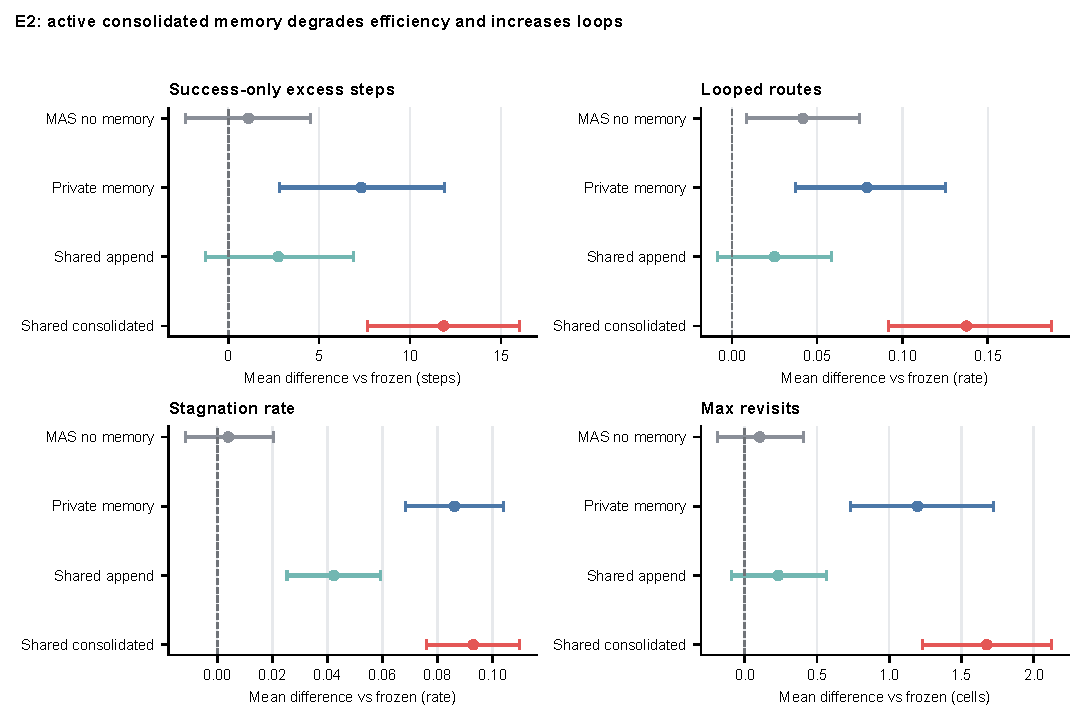
\includegraphics[width=\columnwidth]{figures/beta/figure2_e2_main.pdf}
\caption{\textbf{E2 main result: paired differences versus frozen write-only memory} (five
seeds, final round). Points are mean differences; bars are 95\% bootstrap CIs; the dashed
line is zero. Shared-consolidated (red) degrades on all four endpoints with the largest
effects; MAS-no-memory (grey) sits on the zero line except for a small loop increase.}
\label{fig:fig2}
\end{figure}

Three readings follow. First, multi-agent execution is not itself pathological:
MAS-no-memory matches frozen on efficiency and success, with only a small loop increase
($+0.042$, CI $[0.008, 0.075]$); frozen itself matches no-memory, so this comparison does
not reveal a storage-only effect. Second, \textbf{within this setting, the
shared-consolidated arm meets every preregistered degradation criterion}: success-only excess
steps $+11.84$ (CI $[7.66, 16.02]$), same-sign in $5/5$ seeds; loop rate $+0.138$ (CI
$[0.092, 0.188]$); success $-0.171$. Third, active injection is a broad risk in this
experiment---private memory also degrades---so we test the narrower shared-specific contrast
directly.

\paragraph{Shared versus private boundary.}
The original E2 matrix contrasts the shared arms against a \emph{private} baseline. The
efficiency separation is not significant (consolidated vs.\ private success-only excess steps
$+0.87$, CI $[-4.29, +6.15]$), but loop amplification is: consolidated loops significantly
more than private ($+0.058$, CI $[0.008, 0.113]$), while append loops \emph{less}. The honest
claim is therefore that consensus consolidation specifically amplifies looping relative to
private memory; we do not claim a broad shared-over-private efficiency gap.

\subsection{E3: Read-Side Dose-Response Is Null}

If the harm were read-side---agents increasingly retrieving a few high-vote memories---then
raising the importance weight $\lambda$ in Generative-Agents-style scoring should deepen
degradation. We did not observe that preregistered monotone pattern. Sweeping
$\lambda\in\{0,0.5,1\}$ on the append arm (three seeds,
$T{=}6$), the paired difference of $\lambda{=}1$ versus $\lambda{=}0$ on success-only excess
steps is $+1.69$ (CI $[-4.26, +7.61]$), loop rate $+0.049$ (CI $[0.000, 0.104]$), and
final-round retrieval entropy is non-monotone in $\lambda$ ($0.833/0.826/0.845$). The
read-side usage-weighted-feedback hypothesis is therefore not supported in the tested
$\lambda$ range; this null result is not evidence that every retrieval-side mechanism is
harmless.

\subsection{Mechanism Audit: Write-Side Strategy-Supply Compression}

An offline audit of the same E2 runs locates the concentration on the \emph{write} side
(Figure~\ref{fig:fig3}). Under identical settings, the consolidated pool converges to $14.2$
items with only $11.0$ distinct experiences ever injected across all rounds, whereas the
append pool grows to the cap ($80$) and injects $25.4$ distinct experiences, and private
injects $37.6$. Consensus consolidation compresses the population's active strategy supply
by roughly $2.3\times$ relative to append. The top-1 retrieval share rises in step, but this
is a consequence of the smaller pool rather than an independent channel; the load-bearing
evidence is the direct pool-size and distinct-injection counts. Given the intervention
results below, we report compression as a robust, cross-checked \emph{correlate} and
candidate mechanism, not as established cause.

\begin{figure*}[t]
\centering
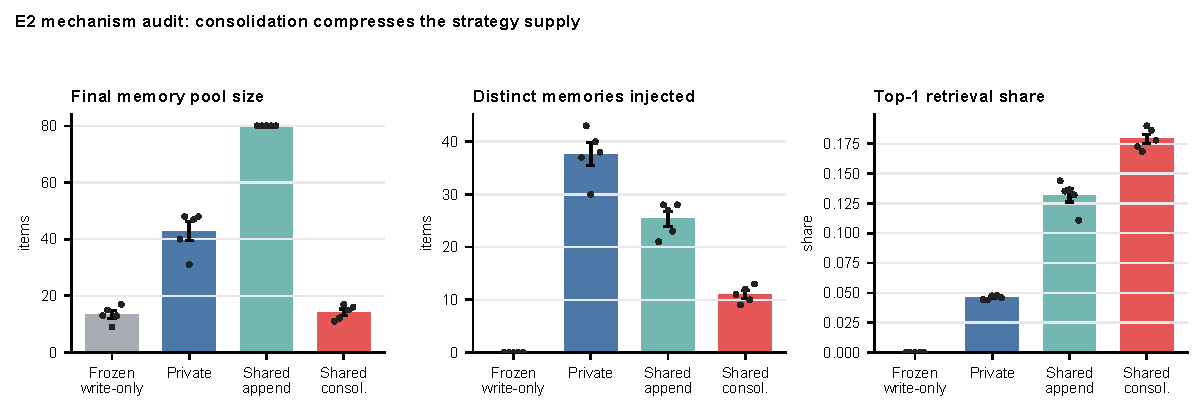
\includegraphics[width=0.92\textwidth]{figures/beta/figure3_write_side_compression.pdf}
\caption{\textbf{Mechanism audit: consolidation compresses the strategy supply.} Final pool
size, distinct experiences ever injected, and top-1 retrieval share across five seeds (dots).
Consensus consolidation keeps a small pool and injects the fewest distinct strategies,
concentrating retrieval; the direct counts (left, centre) carry the claim.}
\label{fig:fig3}
\end{figure*}

\IfFileExists{generated/revision_results/mechanism_controls.tex}{
  \input{generated/revision_results/mechanism_controls.tex}
}{
  \typeout{Fresh mechanism-control table is pending complete formal evidence.}
}

\subsection{E4: Long-Horizon Stress Test (Exploratory)}

We extend the shared arms to $T{=}10$ (three seeds; exploratory). Relative to frozen,
shared-consolidated remains degraded at $t{=}3,6,9$: success differences are
$-0.174/-0.146/-0.257$ and loop differences are $+0.083/+0.083/+0.118$ (all CIs exclude
zero). A within-condition late-versus-early comparison detects no further consolidated
self-trend, so the gap opens early and persists at a noisy plateau rather than provably
deepening. Shared append instead improves over time on cost ratio ($-0.079$), excess steps
($-3.50$), stagnation ($-0.026$), and max revisits ($-0.340$), with all four CIs excluding
zero; this is not a universal append claim. Seed effects remain heterogeneous: seed 1 has
the only detected late success decline, seed 2 ends with the worst trajectory, and seed 0
shows no decline.

\subsection{The Failure Is Silent}

Figure~\ref{fig:fig1}(b) shows a case study mined from the runs: the same held-out maze and
agent at the final round, whose shortest path is 38 steps. As the write protocol
consolidates, the route degrades monotonically---frozen 39 steps (one revisit), private 47
(four), shared-append 55 (nine), shared-consolidated 73 with cost 1.92, eleven revisits to
the same cell, and a detected loop---yet every route is legal and every arm still reaches the
goal. This is the ant-mill signature: not a false belief, but a locally plausible correction
signal, reinforced through consensus writing, that composes into a globally wasteful cycle.

% ============================================================================
\section{Mechanism Interventions and Boundaries}\label{sec:gamma}
% ============================================================================

A second preregistration (Phase Gamma) froze two archive interventions and a cross-model
probe.

\paragraph{Archive interventions.}
The additive arm retains discarded variants and injects active top-6 plus archive top-6.
Distinct supply roughly doubles, but so does prompt dose. No endpoint improves: success
non-inferiority fails ($-0.056$, CI $[-0.153,+0.042]$), success-only excess is null
($-0.45$, CI $[-6.86,+5.96]$), and stagnation worsens ($+0.045$, CI
$[+0.023,+0.067]$). A second arm jointly ranks active and archive candidates under the
original total top-6. Its preregistered diversity-expansion check fails
($1.42/1.55/1.07\times$ across seeds), despite archive selection in $896/912$ eligible
retrievals. We therefore do not evaluate its behavioral gate or claim that equal-dose
archive rescue is ineffective. Added-dose re-exposure can backfire, while one fixed-capacity
joint ranking does not establish restored diversity; compression remains a correlate with an
unresolved causal role.

\subsection{Cross-Model Probe: Compression Replicates, Coupling Is Not Detected}

We repeat the frozen/append/consolidated triangle on Qwen3-32B~\citep{yang2025qwen3}
(three seeds, $T{=}4$). The preregistered gate is
\emph{not-detected-or-underpowered}. Efficiency is direction-consistent but unresolved:
success-only excess is $+5.83$ (CI $[-3.75,+15.20]$, all three seed signs positive).
Loop rate is $-0.076$ (CI $[-0.153,0.000]$), excluding the primary model's
$+0.138$ amplification, and success shows no drop ($+0.042$, CI $[-0.049,+0.132]$).
Yet consolidation still compresses distinct injected supply by $1.55\times$ on Qwen versus
$1.68\times$ on DeepSeek. Similar structural compression with different detected behavior
argues against treating compression alone as sufficient cause. The MiniWoB boundary is
reserved for the main-text transfer display once its formal evidence is complete; full Qwen
diagnostics remain in the artifact.

\IfFileExists{generated/revision_results/miniwob_boundary.tex}{
  \input{generated/revision_results/miniwob_boundary.tex}
}{
  \typeout{MiniWoB boundary table is pending complete formal evidence.}
}

% ============================================================================
\section{Design Implications}
% ============================================================================

\begin{itemize}
\item \textbf{Treat shared consolidation as an audited design choice.} In this setting, the
same infrastructure degrades under reviewer consolidation while the exploratory
$\lambda{=}1$ append arm improves over a longer horizon. Consolidation should therefore be
measured rather than assumed to be hygiene.
\item \textbf{Monitor the write side in addition to success.} Distinct injected experiences,
pool-size trajectory, and retrieval concentration are logged-at-source signals; success alone
can miss efficiency decay.
\item \textbf{Track loops and stagnation in agent telemetry.} Repeated state-action
signatures and stagnation separated consolidated from private memory when aggregate efficiency
did not.
\item \textbf{Do not assume an archive fixes consolidation.} Added-dose re-exposure worsened
stagnation here, while the equal-dose intervention did not meet its diversity manipulation
check. A retained archive must also be retrievable under the deployed ranking rule.
\end{itemize}

% ============================================================================
\section{Limitations}
% ============================================================================

The maze is the only environment in which shortest-path cost and position cycles are known
exactly, and all studies use one primary model, DeepSeek-V3. The six-family MiniWoB boundary
adds executable browser interaction but remains a controlled synthetic benchmark rather than
an open-web or deployment workflow. The Qwen probe bounds but does not establish cross-model
transfer: efficiency is unresolved (underpowered), and the loop signature does not carry at
the primary-model magnitude. Strategy-supply compression also remains a candidate channel.
The exact-size yoke equalizes candidate count but not item content or write history; the MMR
control changes only read selection through deterministic token-hashing cosine; and no
deterministic writer-compression baseline is included. Thus the interventions constrain, but
do not identify, compression as the cause of any behavioral separation. The fresh maze suites
use a seed-clustered hierarchical bootstrap, but the controls and exact yoke have five seeds,
the sensitivity suite has three, and MiniWoB has three seeds per task family. Seed-level
heterogeneity is therefore reported descriptively rather than treated as many independent
replications. Success-only excess steps is conditional on success and must be read jointly
with success and failure-penalized cost. Effects may differ with stronger reviewers, other
consolidation prompts, or retrieval schemes beyond similarity ranking. The MMR control tests
one reproducible lexical diversity policy, not learned semantic MMR, xQuAD, or
diversity-preserving retrieval generally. The private-consolidated control also reallocates
reviewer calls by pool---four per-agent calls versus one joint shared call per training
maze---so it removes cross-agent memory access without isolating sharing from reviewer prompt
composition or total operation opportunity.

% ============================================================================
\section{Conclusion}
% ============================================================================

Shared experiential memory warrants measurement as well as capability evaluation. In a
preregistered maze microscope, the tested shared reviewer-consolidation protocol can reduce
route efficiency, amplify loops relative to private memory, persist over a longer horizon,
and compress the active strategy supply. The archive interventions do not identify
compression as the cause: added-dose re-exposure worsens stagnation, while the equal-dose
intervention fails its preregistered diversity-expansion check. The Qwen probe shows that
compression can transfer without detecting the observed behavioral coupling. The ant-mill is
therefore a bounded
warning, not a claim of universal degradation: locally plausible experience can compose into
globally wasteful behavior.

\paragraph{Reproducibility.}
The anonymized supplementary artifact contains preregistrations with SHA-256 freeze records,
decision logs, per-route artifacts, memory audits, prompts, configurations, statistics code,
and maze runners. Every number in this paper maps to a frozen gate report or an explicitly
labeled exploratory analysis.

\bibliography{antmill_memory}

\end{document}
